\subsection{Tileable Polygons}

\frame{
  \frametitle{Extensions to Tileable Polygons}

  Other Tileable Polygons:

  \begin{columns}
    \begin{column}{0.45\textwidth}
      \begin{figure}
        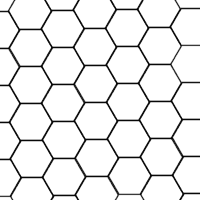
\includegraphics[height=1.5in]{hexagon_tiling.png}
        \caption{Regular Hexagons}
      \end{figure}
    \end{column}
    \begin{column}{0.45\textwidth}
      \begin{figure}
        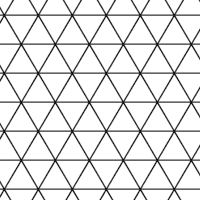
\includegraphics[height=1.5in]{triangle_tiling.png}
        \caption{Equilateral Triangles}
      \end{figure}
    \end{column}
  \end{columns}
}

\subsection{Non-Tileable Polygons}

\frame{
  \frametitle{Extensions to Non-Tileable Polygons}
  \begin{itemize}
    \item Irregular triangles
    \item Pentagons
    \item Octagons
  \end{itemize}
}

\subsection{Circles}

\frame{
  \frametitle{Extensions to Circles}

  \begin{itemize}
    \item Characterize how particle bounces around circle
    \item Analog to $a$, $b$ might be sequence of collision points as you move around circle.
  \end{itemize}

  \begin{figure}
    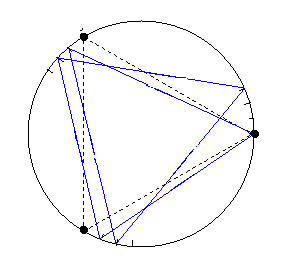
\includegraphics[width=2in]{circle_research.png}
  \end{figure}
}
